\chapter{Implementacja regulatora DMC MIMO oraz przygotowanie odpowiedzi skokowych}

\section{Implementacja DMC}

Dla regulatora DMC $2 \times 2$ r�wnania algorytmu przyjm� nast�puj�c� posta�:

\begin{equation}
y(k) = 
\begin{bmatrix}
y_{1}(\textrm{k}) \\
y_{2}(\textrm{k}) \\
\end{bmatrix}
\end{equation}

\begin{equation}
y^{\text{\textrm{zad}}}(k) = 
\begin{bmatrix}
y_{1}^{\textrm{zad}}(\textrm{k}) \\
y_{2}^{\textrm{zad}}(\textrm{k}) \\
\end{bmatrix}
\end{equation}

\begin{equation}
u(k) = 
\begin{bmatrix}
u_{1}(\textrm{k}) \\
u_{2}(\textrm{k}) \\
\end{bmatrix}
\end{equation}

\begin{equation}
S_l = 
\begin{bmatrix}
s_{l}^{\textrm{11}} & s_{l}^{\textrm{12}} \\
s_{l}^{\textrm{21}} & s_{l}^{\textrm{22}} \\
\end{bmatrix}
,l = 1...D
\end{equation}

\begin{equation}
M = 
\begin{bmatrix}
S_1 & 0 & \hdots & 0 \\
S_2 & S_1 & \hdots & 0 \\
\vdots & \vdots &\ddots & \vdots \\
S_N & S_{N-1} & \hdots & S_{N-N_{\text{u}}+1} \\
\end{bmatrix}
\end{equation}

\begin{equation}
M^{\text{P}} = 
\begin{bmatrix}
S_2-S_1 & S_3-S_2 & \hdots & S_D-S_{D-1} \\
S_3-S_1 & S_4-S_2 & \hdots & S_{D+1}-S_{D-1} \\
\vdots & \vdots & \ddots & \vdots \\
S_{N+1}-S_1 & S_{N+2}-S_2 & \hdots & S_{N+D-1}-S_{D-1} \\
\end{bmatrix}
\end{equation}

\begin{equation}
K = (M^{\textrm{T}}M+\lambda I)^{-1}M^{\textrm{T}} 
\end{equation}

\begin{equation}
Y^\textrm{0}(k) = Y(k)+M^{\textrm{P}} \Delta U^{\textrm{P}}(k)
\end{equation}

\begin{equation}
\Delta U(k) = K( Y^{\textrm{zad}}(k) - Y^\textrm{0}(k) )
\end{equation}

\section{Odpowiedzi skokowe}

\begin{comment}
Jako parametry regulatora DMC zosta�y wybrane odpowiedzi skokowe dla dw�ch oddzielnych zmian warto�ci sterowania $G1$ z \num{18} na \num{38} i $G2$ z \num{23} na \num{43} z punktu pracy. Odpowiedzi skokowe obu wyj�� $T1$ i $T3$ dla skoku $G1$ przedstawiono na rys.~\ref{odp_skok_g1}, a dla skoku $G2$ na rys.~\ref{odp_skok_g2}.

\begin{figure}
	\centering
	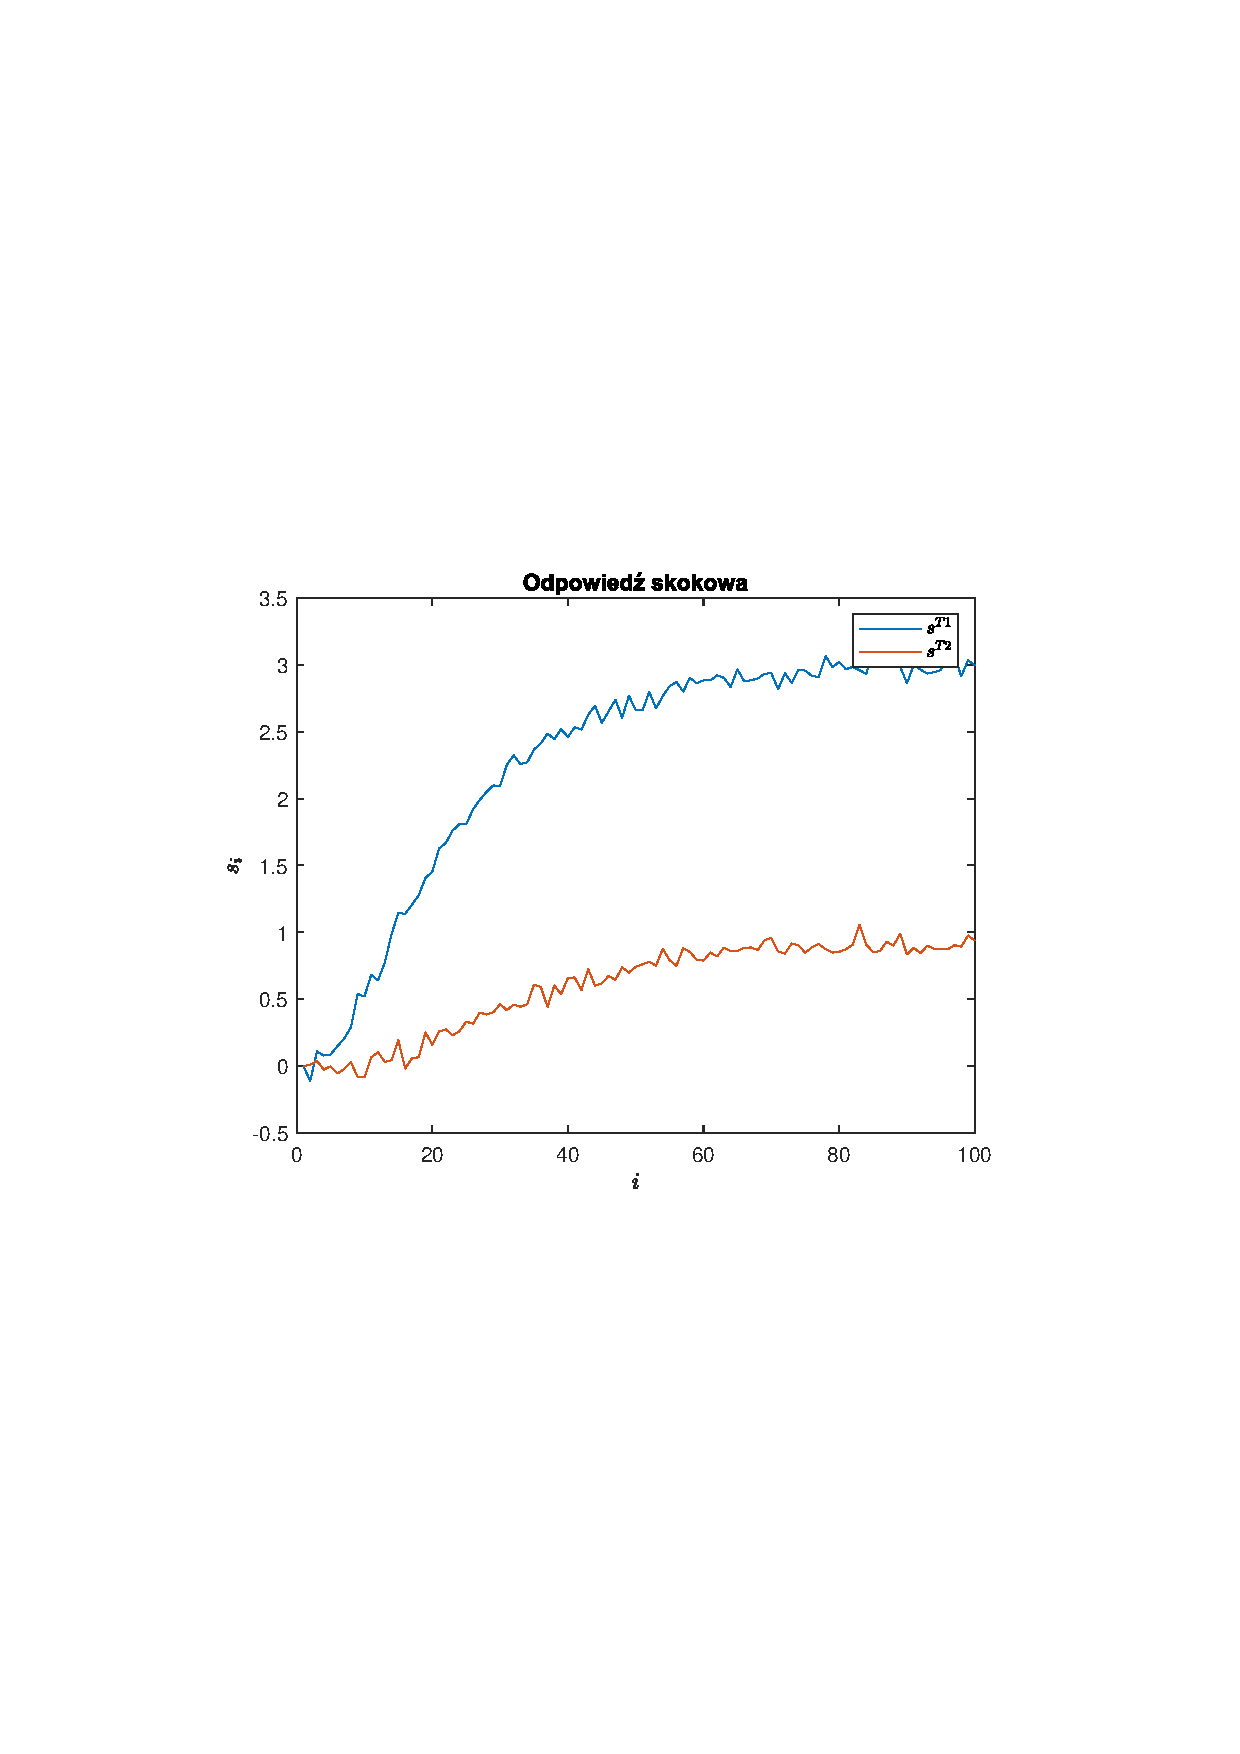
\includegraphics[scale=0.85, trim={2cm 8.5cm 2cm 8.5cm}]{rysunki/odp_skok_g1}
	\caption{Odpowied� skokowa dla zmiany sygna�u sterowania $G1$ z $\num{18}$ na $\num{38}$  z punktu pracy}
	\label{odp_skok_g1}
\end{figure}
\end{comment}

%Aproksymacja?

\subsection{Implementacja}

Do zrealizowania zadania zosta�y u�yte skrypty \verb+zad2.m+ oraz \verb+odp_skok.m+.